\cleardoubleoddpage
\begingroup
\fontsize{11pt}{13.2pt}\selectfont
\chapter{Implementation}
\label{chap:implementation}

We implement the theoretical framework from Chapter~\ref{chap:methodology} as a modular research prototype using modern deep learning frameworks. The implementation covers two experimental tracks: (1) diffusion-based OOD detection on CIFAR-10, and (2) the inkjet print quality classification pipeline. Our architecture emphasises modularity, reproducibility, and extensibility. The implementation leverages PyTorch Lightning~\cite{falcon2019pytorch} for training orchestration, the Hugging Face Diffusers library for diffusion model components, and Hydra~\cite{yadan2019hydra} for flexible configuration management. All code follows standard practices for documentation and reproducibility.

%% ------------------------------------------------------------------

\section{System Overview and Design}
\label{sec:impl:system_overview}

Our implementation consists of five core components: (1) configuration management (Hydra), (2) data loading (PyTorch Lightning \texttt{DataModule}), (3) model definitions (binary conditional diffusion with UNet), (4) training orchestration (Lightning Trainer), and (5) evaluation framework (metrics and OOD detection).

The system design prioritises three principles: \textbf{modularity} (independent components with clear interfaces enabling easy extension), \textbf{configurability} (all hyperparameters externalised in YAML files enabling reproducible experimentation without code modification), and \textbf{reproducibility} (deterministic training through seed management and complete configuration logging). Models inherit from a common base class implementing shared functionality (noise scheduling, loss computation, optimisation), while specific variants (binary conditional UNet for OOD detection, multi-head conditional CDM for inkjet QC) override methods for task-specific behaviour. This inheritance-based design eliminates code duplication while preserving flexibility.

The Hydra configuration system follows hierarchical composition, where base configurations define defaults that can be overridden by experiment-specific settings. For example, a conditional diffusion UNet model can be launched with default settings via \texttt{python train.py}, or customised with: \texttt{python train.py model.learning\_rate=1e-4 trainer.devices=4}. Configuration overrides are automatically logged and saved with results for reproducibility.

%% ------------------------------------------------------------------

\section{CIFAR-10 OOD Detection Implementation}
\label{sec:impl:cifar10_ood}

\subsection{Model Architecture Implementations}
\label{sec:impl:cifar10_model}

\paragraph{Conditional Diffusion with UNet}

The primary model uses the \texttt{UNet2DModel} from the Hugging Face Diffusers library with the following configuration: 3 input channels (RGB), \texttt{block\_out\_channels=(128, 256, 256, 512)} (base channel 128 with multipliers $[1, 2, 2, 4]$), attention at resolutions $[16, 8]$, 2 residual blocks per resolution, and 512-dim embeddings for both timestep and class (in contrast to the 256-dim embeddings used in the inkjet pipeline). Class information is incorporated through learnt embeddings injected via adaptive group normalisation (AdaGN) layers at multiple scales.

Training uses AdamW optimisation (learning rate $10^{-4}$, weight decay $\lambda_{\text{wd}} = 0.01$) with cosine annealing and a 5-epoch linear warm-up, effective batch size 128 (batch 64 with gradient accumulation $\times 2$), and up to 200 epochs on CIFAR-10 (early stopping, patience=30 on validation AUROC; typical convergence at epoch 15--25). For the binary CDM experiments, conditioning is reduced to two classes (airplane as ID, remaining nine classes as OOD), yielding a model of approximately 68.8M parameters (verified by direct parameter count of the instantiated \texttt{ConditionalUNet} using the training-run configuration logged in W\&B).

\subsection{CIFAR-10 Data Pipeline}
\label{sec:impl:cifar10_data}

Data loading uses PyTorch Lightning's \texttt{LightningDataModule} abstraction enabling seamless dataset switching. CIFAR-10 is split into 45K training, 5K validation, and 10K test sets with standard augmentation (horizontal flip). The retained external OOD datasets (CIFAR-100, Places365, FashionMNIST, SVHN, Textures) undergo identical preprocessing (normalisation to $[-1, 1]$) without augmentation during evaluation. FashionMNIST images are resized from $28 \times 28$ to $32 \times 32$ and converted from greyscale to 3-channel RGB.

\subsection{OOD Evaluation Pipeline}
\label{sec:impl:cifar10_eval}

Evaluation computes reconstruction error by sampling $K$ random timesteps for each test image, following Algorithm~\ref{alg:ood_evaluation} in Chapter~\ref{chap:methodology}. All metrics (AUROC, FPR@95\%TPR, accuracy) use scikit-learn implementations. W\&B logging tracks metrics per epoch, and model checkpoints are saved at best validation loss and best OOD AUROC.

%% ------------------------------------------------------------------

\section{Inkjet Quality Control Implementation}
\label{sec:impl:inkjet_qc}

The inkjet quality control pipeline extends the CIFAR-10 OOD framework to a practical industrial setting. This section describes the implementation of each pipeline component: the YOLOv8 feature detector, the multi-condition CDM, and the comparison methods.

\subsection{YOLOv8 Feature Detector}
\label{sec:impl:yolov8}

\paragraph{Model Selection}

We use YOLOv8n (nano), the smallest variant with $\sim$3.2M parameters, which provides sufficient detection accuracy for our well-structured template images while enabling fast inference. The model is trained on the thesis feature annotations and accessed through the Ultralytics library.

\paragraph{Training Configuration}
\begin{itemize}
\item Input resolution: $640 \times 640$ (standard YOLO input)
\item Epochs: 100 with early stopping (patience 20)
\item Optimiser: SGD with momentum 0.937, weight decay 0.0005
\item Learning rate: 0.01 with cosine annealing
\item Augmentation: mosaic, mixup, flip, HSV colour jitter
\end{itemize}

\paragraph{Detection Output}

For each template image, the detector outputs bounding boxes $[x_{\min}, y_{\min}, x_{\max}, y_{\max}]$, class predictions (8 feature types), and confidence scores. Only detections with confidence $> 0.3$ are retained. The expected number of detections per template ranges from 2 to 5 depending on the template type, yielding an average of $\sim$4.8 features per image across the dataset.

\paragraph{Feature Extraction}

Each detected region is cropped from the original $1920 \times 1080$ image and resized to $128 \times 128$ pixels using bilinear interpolation. The crop coordinates, feature class, and template type are stored as metadata for downstream CDM conditioning.


\subsection{Conditional Diffusion Model for Quality Classification}
\label{sec:impl:inkjet_cdm}

\paragraph{Architecture}

The inkjet CDM uses a custom \texttt{NoisePredictorV3} UNet (not \texttt{UNet2DModel}) tailored for $128 \times 128$ input with multi-head conditioning:
\begin{itemize}
\item Input channels: 3 (RGB)
\item Base channels: 64
\item Channel multipliers: $[1, 2, 4, 8]$ (effective block channels 64, 128, 256, 512)
\item Attention at resolutions: $[32, 16]$
\item Residual blocks per level: 2
\item Total parameters: $\sim$9.3M (verified by direct parameter count of the \texttt{NoisePredictorV3} module with \texttt{base\_channels=64})
\end{itemize}

\paragraph{Multi-Head Conditioning Implementation}

The four conditioning heads (Section~\ref{sec:meth:inkjet:multihead}) are implemented as follows:
\begin{itemize}
\item Template embedding: \texttt{nn.Embedding(3, 256)} encodes template type (A/B/C) into a 256-dim vector
\item Feature embedding: \texttt{nn.Embedding(8, 256)} encodes feature type into a 256-dim vector
\item Quality embedding: \texttt{nn.Embedding(2, 256)} encodes the GOOD/BAD label into a 256-dim vector
\item Bbox encoder: \texttt{nn.Sequential(Linear(4, 64), GELU, Linear(64, 256))} encodes normalised bounding box coordinates
\item Timestep embedding: standard sinusoidal encoding $\to$ MLP $\to$ 256-dim vector
\end{itemize}

All five embeddings are summed to produce the final conditioning vector $c \in \mathbb{R}^{256}$, which is injected via AdaGN at each UNet resolution level.

\paragraph{Training Details}
\begin{itemize}
\item Optimiser: AdamW ($\text{lr} = 2 \times 10^{-4}$, weight decay $= 10^{-4}$)
\item Batch size: 128 for the $\lambda=0$ baseline and 64 for $\lambda>0$ runs with separation loss
\item Noise schedule: Cosine, $T = 1000$
\item Training: 100 epochs per fold
\item Hardware: Single GPU per run (V100 16\,GB, GV100 32\,GB, or P40 24\,GB depending on availability); training time $\sim$6--8\,h per fold on V100, comparable on GV100/P40
\end{itemize}

\paragraph{Inference}

Quality classification follows Algorithm~\ref{alg:quality_classification}. The public implementation defaults to $K = 50$ Monte Carlo trials per sample, while the retained 5-fold cross-validation ablation reported in Chapter~\ref{chap:results} uses $K = 100$ for more stable estimates. For each trial, a random timestep $t \sim \mathcal{U}[1, 1000]$ and noise $\epsilon \sim \mathcal{N}(0, I)$ are sampled. The model predicts noise under both GOOD and BAD conditions, and the class with lower reconstruction error is selected as the prediction.

\subsection{Comparison Method Implementations}
\label{sec:impl:inkjet:comparisons}

\paragraph{Retained public comparison scope.}
Earlier internal experiments considered supervised and anomaly-detection baselines, but those non-CDM pipelines are not retained as thesis evidence because their full public code, splits, configurations, and result artefacts are not part of the released package. The implementation described here therefore focuses on the public YOLO+CDM pipeline that can be reproduced from \texttt{InkjetOOD}, the public FTI\_Zer0P dataset, and the released inkjet CDM weights.


\subsection{Public Inkjet Evaluation Infrastructure}
\label{sec:impl:comparison_methods}

The public inkjet implementation retained in this thesis is the
\texttt{InkjetOOD} CDM pipeline together with its training, evaluation,
ablation, and 5-fold cross-validation scripts.

\paragraph{Public CDM Components}
\begin{itemize}
\item \textbf{Training entry point}: \texttt{train.py} reproduces the multi-head CDM training run for a chosen separation-loss weight.
\item \textbf{Evaluation entry point}: \texttt{evaluate.py} reproduces GOOD-vs.-BAD scoring with configurable $K$ Monte Carlo trials.
\item \textbf{Ablation script}: \texttt{run\_ablation.py} evaluates $\lambda \in \{0.0, 0.01, 0.02, 0.05\}$ under a shared train/test split.
\item \textbf{Cross-validation script}: \texttt{run\_cv.py} runs the retained 5-fold image-level protocol and writes fold summaries used in Chapter~\ref{chap:results}.
\end{itemize}

\subsection{Cross-Validation Infrastructure}
\label{sec:impl:cross_validation}

\paragraph{Stratified 5-Fold Cross-Validation}

The retained public CDM experiments use image-level splitting rather than
sample-level splitting, preventing data leakage from correlated crops
derived from the same template image.

\paragraph{Splitting Algorithm}
\begin{enumerate}
\item Group samples by processed source image (573 groups)
\item Stratify groups by quality label distribution
\item Split groups into 5 folds with balanced label ratios
\item Expand folds to sample level for training and evaluation
\end{enumerate}

This ensures that each fold has a representative distribution of all template types, feature types, and quality labels.

\begin{figure}[htbp]
\centering
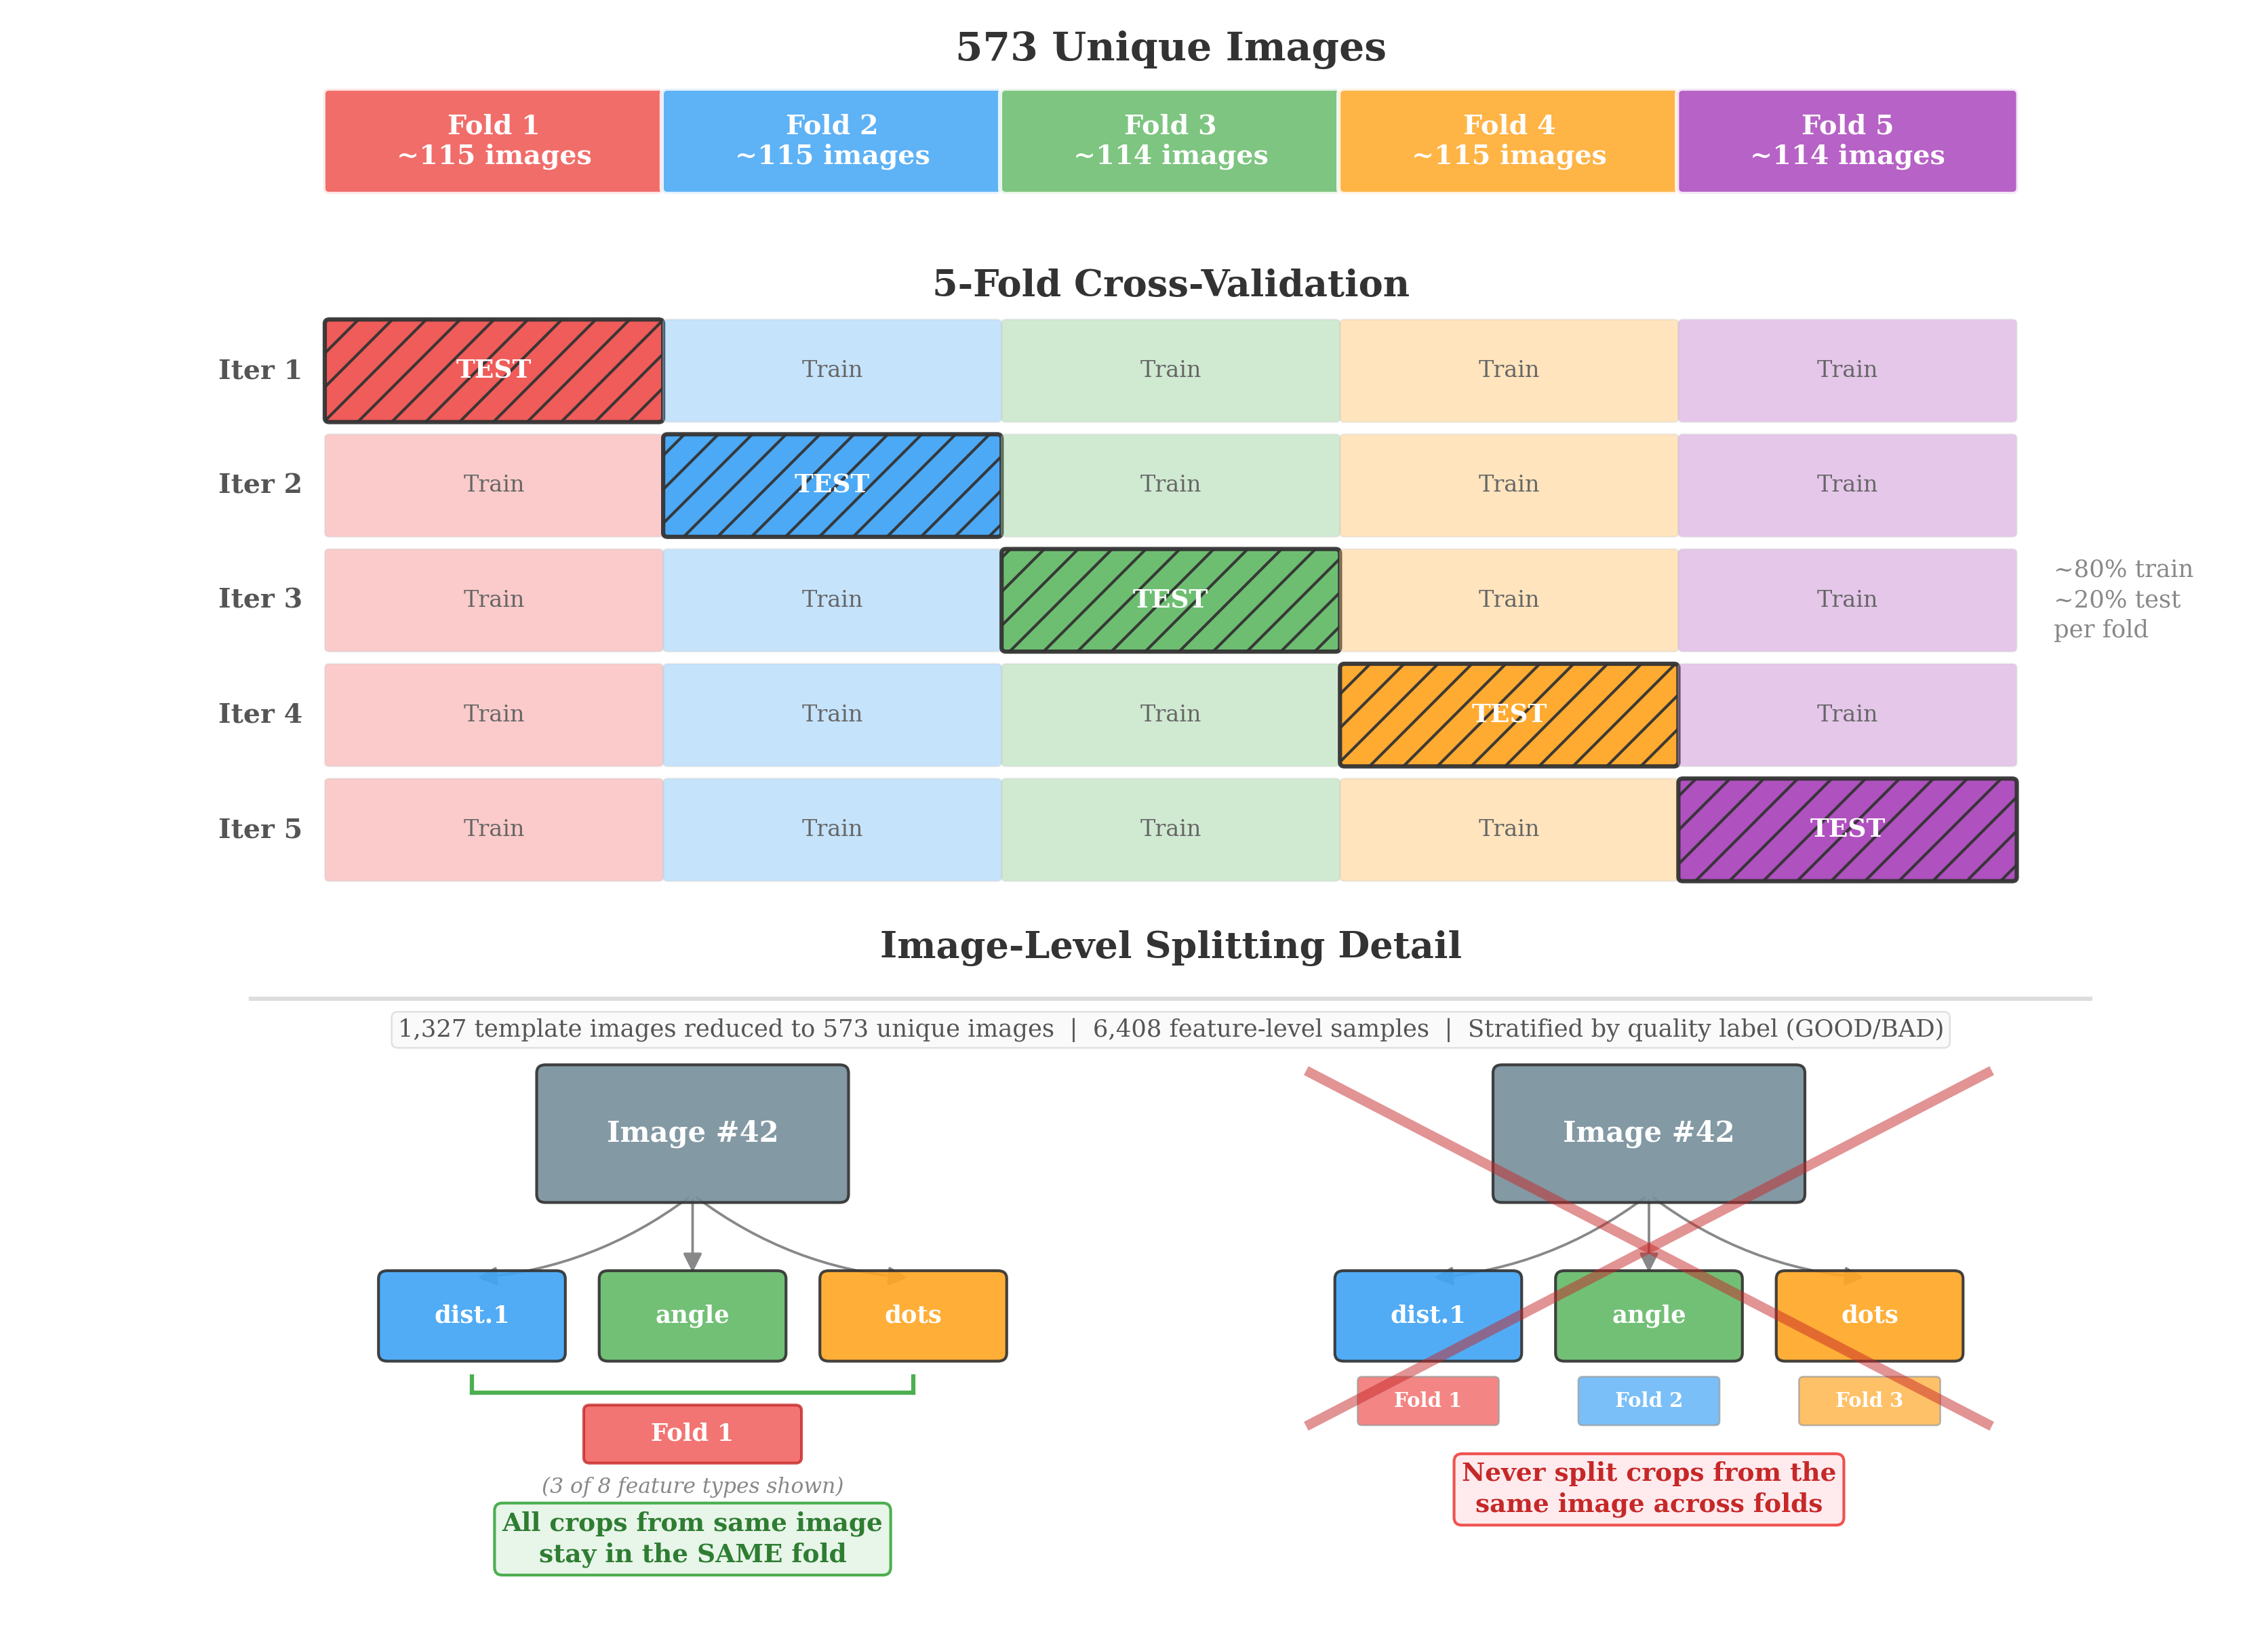
\includegraphics[width=\textwidth]{images/fig_cross_validation.png}
\caption{Stratified 5-fold cross-validation with image-level splitting. The 573 processed source-image groups are partitioned into 5 folds (114--115 groups per fold), with each fold serving as the test set exactly once. Bottom: image-level splitting ensures all feature crops derived from the same source image remain in the same fold, preventing data leakage between training and test sets.}
\label{fig:cross_validation}
\end{figure}

%% ------------------------------------------------------------------

\section{Key Engineering Considerations}
\label{sec:impl:engineering}

\paragraph{Memory Efficiency}

Training across the available GPU pool (V100 16\,GB, GV100 32\,GB, P40 24\,GB) requires careful memory management. We use mixed-precision (AMP) training, reducing peak activation memory to $\approx$4--6\,GB and enabling execution even on the V100 (16\,GB, the tightest available GPU), enable gradient accumulation to maintain effective batch sizes with smaller per-GPU batches, and implement efficient data loading with 8 worker processes and pinned memory.

\paragraph{Inference Cost}

OOD detection requires multiple forward passes ($K$ timesteps per image). For the binary CDM setup measured on an NVIDIA GeForce RTX 2080 Ti, $K = 50$ takes 4861.1\,s ($\sim$81.0 minutes) per 10K images, about $492\times$ the measured ResNet-18 wall-clock cost on the same hardware. With $K = 10$, inference takes 972.9\,s ($\sim$16.2 minutes; $68.6\times$ ResNet-18 cost) while maintaining 98.2\% AUROC in the binary setup. $K = 1$ achieves 91.0\% AUROC but was not re-timed in the final consistency pass, so no wall-clock ratio is claimed for it. These $K$ ablation timings use the seed-42 $\lambda=0.01$ checkpoint. For the inkjet pipeline, inference takes $\sim$0.5 seconds per feature crop with $K = 50$ trials.

\paragraph{Reproducibility Measures}

All retained experiments use fixed random seeds with PyTorch deterministic mode enabled. Configuration files, git commit hashes, and environment metadata (Python/CUDA versions) are logged automatically. Public reproduction relies on the released repositories, weights, raw scores, configuration files, and command sequences summarised below and in Appendix~\ref{app:experimental-config}.

\paragraph{Multi-GPU Training}

The code supports PyTorch Lightning's DDP (Distributed Data Parallel) with automatic gradient synchronisation, but all reported thesis experiments use a single GPU per run. Multi-GPU training is therefore an implementation capability rather than part of the reported experimental protocol.

%% ------------------------------------------------------------------

\section{Reference Implementation}
\label{sec:impl:reference_impl}

\noindent\textbf{CL-2 Reproducibility.}
The CIFAR-10/OOD implementation is publicly available at \url{https://github.com/ahmed-3m/DiffusionOOD}, with weights at \url{https://huggingface.co/ahmed-3m/DiffusionOOD}. The inkjet CDM implementation, experiment documentation, and figure-generation scripts are publicly available at \url{https://github.com/ahmed-3m/InkjetOOD}~\cite{mohammed2026inkjetood}, with weights at \url{https://huggingface.co/ahmed-3m/InkjetOOD}; the accompanying FTI\_Zer0P dataset is available from Zenodo at DOI~\href{https://doi.org/10.5281/zenodo.11444566}{10.5281/zenodo.11444566}~\citep{profactor2024fti}. The codebases follow standard PyTorch~\cite{paszke2019pytorch} project layouts with modules for models, data loading, evaluation, training scripts, and configuration. Key software dependencies and versions are listed in Appendix~\ref{app:dependencies}.
\endgroup
